\section{Optimasi Lanjut dan Peran SSA}

Bentuk \compiler{Static Single Assignment (SSA)} telah merevolusi cara kompilator melakukan optimasi, termasuk alokasi register.

\subsection{Dampak SSA terhadap Graf Interferensi}
Dalam bentuk SSA, setiap variabel hanya didefinisikan satu kali. Hal ini memiliki beberapa properti menarik bagi pengalokasi register:
\begin{itemize}
    \item \textbf{Chordal Graphs}: Graf interferensi yang dihasilkan dari kode berbasis SSA seringkali bersifat \textit{chordal}. Untuk graf jenis ini, masalah pewarnaannya tidak lagi NP-Complete dan dapat diselesaikan dalam waktu polinomial untuk hasil yang optimal.
    \item \textbf{Liveness Analysis}: Properti SSA menyederhanakan perhitungan rentang hidup variabel (\textit{live ranges}) karena tidak ada ambiguitas definisi variabel.
\end{itemize}

\subsection{Penamaan Ulang Register (Register Renaming)}
\textit{Register Renaming} pada tingkat perangkat lunak (kompilator) bertujuan menghilangkan ketergantungan semu (\textit{WAR - Write-After-Read} dan \textit{WAW - Write-After-Write}).
\begin{itemize}
    \item Dengan menggunakan nama variabel yang berbeda untuk setiap definisi (seperti pada SSA), kompilator memberi kebebasan lebih bagi pengalokasi register untuk menggunakan register yang berbeda, sehingga meningkatkan potensi eksekusi paralel.
\end{itemize}

\begin{figure}[!htbp]
    \centering
    \adjustbox{max width=0.8\textwidth,center}{%
    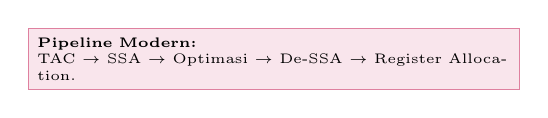
\begin{tikzpicture}[
        node/.style={rectangle, draw=purple!50, fill=purple!10, text width=6cm, font=\tiny}
    ]
    \node[node] (ssa) {
        \textbf{Pipeline Modern:}\\
        TAC $\rightarrow$ SSA $\rightarrow$ Optimasi $\rightarrow$ De-SSA $\rightarrow$ Register Allocation.
    };
    \end{tikzpicture}%
    }
    \caption{Peran SSA sebagai pondasi optimasi dan alokasi register}
\end{figure}
